\documentclass[master=cws,masteroption=ai,fleqn,english]{kulemt}
%
% Indien je UTF-8 karakters gebruikt, verwijder "% " uit de volgende lijn
\setup{inputenc=utf8,
% Vul de titel van jouw masterproef hieronder in tussen { en }.
title={Distributed Adversarial Attacks},
%
% Vul hieronder namen in, steeds Voornaam Naam.
% Indien meerdere auteurs, assessoren, assistenten, scheidt hun namen met "\and ".
author={Sander Prenen},
promotor={Prof. dr. ir. W. Joosen \and Dr. ir. D. Preuveneers},
assessor={Ir.\,W. Eetveel\and W. Eetrest},
assistant={V. Rimmer \and I. Tsingenopoulos}
}


% Kies de fonts voor de gewone tekst, bv. Latin Modern
\setup{font=lm}

% Hier kun je dan nog andere pakketten laden of eigen definities voorzien
\usepackage{amsmath, amssymb}
\setlength{\mathindent}{1cm}
\setlength{\parindent}{0mm}
\usepackage{tikz}
\usetikzlibrary{positioning}

\usepackage{pgfplots}
\pgfplotsset{compat=1.16}
%\usepgfplotslibrary{external}
%\tikzexternalize

\usepackage[acronym]{glossaries}
\makenoidxglossaries
\newacronym{ai}{AI}{Artificial Intelligence}
\newacronym{ba}{BA}{Boundary Attack}
\newacronym{bba}{BBA}{Biased Boundary Attack}
\newacronym{relu}{ReLU}{Rectified Linear Unit}
\newacronym{ann}{ANN}{Artificial Neural Network}
\newacronym{cnn}{CNN}{Convolutional Neural Network}
\newacronym{rnn}{RNN}{Recurrent Neural Network}
\newacronym{dnn}{DNN}{Deep Neural Network}
\newacronym{svm}{SVM}{Support Vector Machine}
\newacronym{api}{API}{Application Programming Interface}
\newacronym{fgsm}{FGSM}{Fast Gradient Sign Method}
\newacronym{pso}{PSO}{Particle Swarm Optimization}
\newacronym{ea}{EA}{Evolutionary Algorithm}
\newacronym{dknn}{DkNN}{Deep k-Nearest Neighbors}

% Tenslotte wordt hyperref gebruikt voor pdf bestanden.
% Dit mag verwijderd worden voor de af te drukken versie.
\usepackage[pdfusetitle,colorlinks,plainpages=false]{hyperref}

%
%%%%%%%%% Wijzig niets onder deze regel %%%%%%%%

\begin{document}

\begin{preface}

\end{preface}
\begin{abstract}
% Adversarial examples
% Defense
% New attack
% More evasive
%Adversarial attacks craft small perturbations that can be added to inputs, so that they are classified incorrectly by a classifier. Current defensive schemes try to flag these attacks based on the similarity between successive submitted queries. This work aims to implement a new adversarial attack that is able to bypass this detection mechanism. This attack is called PSO-BBA after the two constituent algorithms Particle Swarm Optimization and Biased Boundary Attack \cite{brunner_guessing_2019}. Other improvements, such as distributing the query submission over multiple nodes or grouping attacks together have been explored as well. The final attack is more evasive than current state-of-the-art attacks, but is slightly less efficient. The attacker has to make a trade-off depending on the primary goal of the attack.
Image classification models are prone to adversarial examples. Adversarial examples are perceptually identical to original inputs, but they are classified differently. The examples are crafted using adversarial attack algorithms. Current defensive schemes try to flag these attacks based on the similarity between successive submitted queries. The scheme assumes that it can trace back the origin of every query to a user and that there is no cooperation possible between users. This works aims to exploit these assumptions by implementing a new family of adversarial attacks that uses distributed query submission. This tricks the defensive scheme into thinking that the queries originate from different users. The attack is called PSO-BBA after the two constituent algorithms Particle Swarm Optimization and Biased Boundary Attack \cite{brunner_guessing_2019}. The main advantage of PSO are the different starting points for the algorithm. Different distribution schemes were explored, but none of them proved to be a significant winner. In order to increase the evasiveness, the insertion of other (benign) queries was considered, but this approach proved to hamper the efficiency too much. The insertion of queries originating from other concurrent attacks did improve the evasiveness without an added efficiency cost. The final attack is more evasive than current state-of-the-art attacks, but is slightly less efficient, making it a viable candidate if the cost of detection is high.
\end{abstract}
\tableofcontents
\listoffigures
\listoftables
\printnoidxglossary[type=\acronymtype, title=List of Abbreviations]


\mainmatter
\chapter{Introduction}
% General classification (daunting)
% Neural networks
% DNN
% Adversarial attacks
% Defenses
% Bypass
% Overview
One of the most basic tasks in \gls{ai} or more specifically \gls{ml} is the classification of data. This task is usually performed by a classifier or model based on features present in this data. Some examples of classification tasks are: character recognition \cite{mnist}, spam detection \cite{spambase} and face recognition \cite{face_recognition_survey}. These tasks are generally very daunting for humans causing a great interest in improving the accuracies of these classifiers.\\

The first classifiers made use of algorithms such as nearest neighbors \cite{nearest_neighor}, decision trees \cite{decision_tree} and \glspl{svm} \cite{svm}. More recent classifiers are based on neural networks, which in turn are inspired by the human brain. These networks come in a great variety of forms and show near-human performance on some very specific tasks \cite{alpha_go_google}. This improvement in performance caused even more interest in the applications of \gls{ai} and \gls{ml}. Forbes \cite{forbes} recently predicted that in ten years \gls{ai} will be present in all areas of our society. The next decade is deemed as the \textit{"most promising era in technology innovation"} \cite{forbes}.\\

The prevalence of \gls{ml} in the near future does not only bring opportunities. It also poses some threats that may not be obvious at first glance. A spam email passing through an \gls{ai}-based spam filter might not be the end of the world, while mispredicting some characters from an image can have a bigger impact depending on the context. False predictions in the medical domain might be even more severe, but they could be overturned by a doctor. Self-driving cars not detecting traffic signs could put several lives at risk. Depending on the situation in which the classifier is deployed, some threats can be more dangerous than others.\\

All previous examples of threats are due to the inaccuracies of the classifier itself. There are also some threats caused by the inherent nature of neural networks. In 2014, it was shown that neural networks are prone to adversarial examples \cite{szegedy2014intriguing}. An adversarial example consists of a correctly classified data instance and a small perturbation. This perturbation causes the neural network to misclassify the instance. This allows malicious users to create images that are seemingly identical, while being classified differently. This poses an even greater threat to the security of \gls{ai} than the inaccuracies of the classifiers.\\

The process of creating an adversarial example is called an adversarial attack. Different types of attacks exist depending on the information available to the attacker. White-box attacks require complete knowledge of the classifier under attack, while black-box attacks only require the output(s) of the model. All attacks require sending one or more queries to the classifier.\\

Ever since the discovery of adversarial examples, an arms race between adversarial attack and defense researchers has been taken place. In the current state of affairs in the adversarial \gls{ml} domain, the stateful defensive mechanism \cite{chen_stateful_2019} is considered the state-of-the-art. Unlike previous defensive schemes, this scheme holds state of previously submitted queries. This allows the scheme to make a decision based on a series of queries instead of a single query.\\

The stateful defense mechanism makes the assumption that there is no collaboration between different users of the model and that every submitted query can be traced back to the submitting user. This is not necessarily the case in real scenarios, since users are free to work together. It is even possible for one user to set up multiple accounts and essentially collaborate with itself. This work aims to exploit the assumption made by the defensive mechanism and create adversarial examples while triggering as few detections as possible.\\

This goal is achieved by first altering an existing adversarial attack using \gls{pso} in order to bypass the stateful defense mechanism. \gls{pso} is an optimization framework inspired by the flocking of birds. Afterwards multiple ideas are explored in an effort to improve the efficiency or evasiveness of the altered attack. Some ideas are specific for the created attack, while others are generally applicable to all other adversarial attacks.\\

The work is structured as follows: Chapter \ref{chap:background} discusses the necessary background needed in order to comprehend the rest of the work. Chapter \ref{chap:related_work} gives an overview of work related to this subject. Some specific adversarial attacks are discussed as is the stateful defense mechanism. Chapter \ref{chap:approach} introduces the main ideas used in the development of the altered attack. This chapter also poses some interesting research questions. Chapter \ref{chap:evaluation} proposes a novel attack and iteratively refines this attack in order to increase the efficiency or evasiveness. At the end of every section of this chapter, some conclusions are drawn and discussed. Chapter \ref{chap:discussion} contains a discussion about the work as a whole. Some final remarks are given as well as some pointers for future work. Finally, Chapter \ref{chap:conclusion} concludes this work by answering the research questions posed in Chapter \ref{chap:approach}. \\ 
\chapter{Background}
\section{Neural networks}
Ever since the invention of computer systems, it has always been a goal of scientists and engineers to create \gls{ai}. Current state of the art approaches are mimicking the human brain, more specifically the neurons inside the brain. Already in the fifties, Rosenblatt introduced his perceptron \cite{rosenblatt_perceptron_1958}. The perceptron is a single neuron able to learn linearly separable patterns. It does so by finding a hyperplane that separates the two classes. This hyperplane is called the decision surface or decision boundary and the perceptron itself is called a classifier. Geometric regions separated by a decision boundary are called decision regions. The concept of linear separability is explained in Figure \ref{fig:linear_separability} in two dimensions. In Figure \ref{fig:decision_boundaries_decision_regions}, the decision boundaries and decision regions are explained visually. \\

Unfortunately not all patterns are linearly separable. To overcome this problem, the neurons can be layered, creating an \gls{ann} in the process. Layering neurons sequentially is essentially a linear combination of neurons. This in itself does not create non-linear decision surfaces. Non-linear activation functions are added for the \gls{ann} to be able to learn more complex decision boundaries. Some commonly used activation functions are \gls{relu} \cite{relu}, Heaviside step function and softmax (or sigmoid when used on scalars). In Figure \ref{fig:activation_functions} the plots of the activation functions can be found.\\ 

The neurons can be combined in different ways to create different \gls{ann} architectures. Each architecture has its own strengths and weaknesses. \glspl{cnn} excel in classifying visual data \cite{cnn_1, cnn_2}, whilst \glspl{rnn} are widely used when there exist dependencies inside the data, such as in speech recognition \cite{speech_1, speech_2} or time series prediction \cite{time_series_1}. More recent research focuses on \glspl{dnn}, due to the ever increasing computational power available. \gls{dnn} approaches are able to compare to and even surpass human performance \cite{alpha_go_google, imagenet_dnn}.\\ 

\begin{figure}
\tikzset{every picture/.style={line width=0.75pt}} %set default line width to 0.75pt        
\centering
\begin{tikzpicture}[x=0.75pt,y=0.75pt,yscale=-1,xscale=1]
%uncomment if require: \path (0,300); %set diagram left start at 0, and has height of 300

%Straight Lines [id:da34928766651876697] 
\draw [line width=1.5]    (40,220) -- (190,220) ;
%Straight Lines [id:da5068123062544778] 
\draw [line width=1.5]    (40,120) -- (40,220) ;
%Straight Lines [id:da02959929373017789] 
\draw [color={rgb, 255:red, 247; green, 0; blue, 0 }  ,draw opacity=1 ]   (71,133) -- (81,133) ;
%Straight Lines [id:da023175201693992564] 
\draw [color={rgb, 255:red, 65; green, 117; blue, 5 }  ,draw opacity=1 ]   (132,166) -- (142,166) ;
%Straight Lines [id:da12599178724449778] 
\draw [color={rgb, 255:red, 65; green, 117; blue, 5 }  ,draw opacity=1 ]   (137,161) -- (137,171) ;

%Straight Lines [id:da014209875608111044] 
\draw [color={rgb, 255:red, 65; green, 117; blue, 5 }  ,draw opacity=1 ]   (95,185) -- (105,185) ;
%Straight Lines [id:da8046955093022794] 
\draw [color={rgb, 255:red, 65; green, 117; blue, 5 }  ,draw opacity=1 ]   (100,180) -- (100,190) ;

%Straight Lines [id:da8257858393303268] 
\draw [color={rgb, 255:red, 65; green, 117; blue, 5 }  ,draw opacity=1 ]   (151,177) -- (161,177) ;
%Straight Lines [id:da9904899777355851] 
\draw [color={rgb, 255:red, 65; green, 117; blue, 5 }  ,draw opacity=1 ]   (156,172) -- (156,182) ;

%Straight Lines [id:da4558392192767111] 
\draw [color={rgb, 255:red, 65; green, 117; blue, 5 }  ,draw opacity=1 ]   (132,189) -- (142,189) ;
%Straight Lines [id:da6277106773918533] 
\draw [color={rgb, 255:red, 65; green, 117; blue, 5 }  ,draw opacity=1 ]   (137,184) -- (137,194) ;

%Straight Lines [id:da6088809310233947] 
\draw [color={rgb, 255:red, 65; green, 117; blue, 5 }  ,draw opacity=1 ]   (131,142) -- (141,142) ;
%Straight Lines [id:da9717175839575936] 
\draw [color={rgb, 255:red, 65; green, 117; blue, 5 }  ,draw opacity=1 ]   (136,137) -- (136,147) ;

%Straight Lines [id:da05579332834233042] 
\draw [color={rgb, 255:red, 247; green, 0; blue, 0 }  ,draw opacity=1 ]   (84,146) -- (94,146) ;
%Straight Lines [id:da9339907902154778] 
\draw [color={rgb, 255:red, 247; green, 0; blue, 0 }  ,draw opacity=1 ]   (64,181) -- (74,181) ;
%Straight Lines [id:da801343700133325] 
\draw [color={rgb, 255:red, 247; green, 0; blue, 0 }  ,draw opacity=1 ]   (103,127) -- (113,127) ;
%Straight Lines [id:da6207217857469742] 
\draw [color={rgb, 255:red, 247; green, 0; blue, 0 }  ,draw opacity=1 ]   (58,157) -- (68,157) ;

%Straight Lines [id:da9774802467048496] 
\draw [line width=1.5]    (238,221) -- (388,221) ;
%Straight Lines [id:da8926029470752344] 
\draw [line width=1.5]    (238,121) -- (238,221) ;
%Straight Lines [id:da391932663930169] 
\draw [color={rgb, 255:red, 247; green, 0; blue, 0 }  ,draw opacity=1 ]   (360,200) -- (370,200) ;
%Straight Lines [id:da45698367355392255] 
\draw [color={rgb, 255:red, 65; green, 117; blue, 5 }  ,draw opacity=1 ]   (330,167) -- (340,167) ;
%Straight Lines [id:da8509197980874896] 
\draw [color={rgb, 255:red, 65; green, 117; blue, 5 }  ,draw opacity=1 ]   (335,162) -- (335,172) ;

%Straight Lines [id:da46487388742354385] 
\draw [color={rgb, 255:red, 65; green, 117; blue, 5 }  ,draw opacity=1 ]   (293,186) -- (303,186) ;
%Straight Lines [id:da6402947556346299] 
\draw [color={rgb, 255:red, 65; green, 117; blue, 5 }  ,draw opacity=1 ]   (298,181) -- (298,191) ;

%Straight Lines [id:da371430190479477] 
\draw [color={rgb, 255:red, 65; green, 117; blue, 5 }  ,draw opacity=1 ]   (349,178) -- (359,178) ;
%Straight Lines [id:da029152498087926304] 
\draw [color={rgb, 255:red, 65; green, 117; blue, 5 }  ,draw opacity=1 ]   (354,173) -- (354,183) ;

%Straight Lines [id:da7641303373625803] 
\draw [color={rgb, 255:red, 65; green, 117; blue, 5 }  ,draw opacity=1 ]   (330,190) -- (340,190) ;
%Straight Lines [id:da8503441823041022] 
\draw [color={rgb, 255:red, 65; green, 117; blue, 5 }  ,draw opacity=1 ]   (335,185) -- (335,195) ;

%Straight Lines [id:da14090483844456858] 
\draw [color={rgb, 255:red, 65; green, 117; blue, 5 }  ,draw opacity=1 ]   (329,143) -- (339,143) ;
%Straight Lines [id:da10211881619757635] 
\draw [color={rgb, 255:red, 65; green, 117; blue, 5 }  ,draw opacity=1 ]   (334,138) -- (334,148) ;

%Straight Lines [id:da8074255152632699] 
\draw [color={rgb, 255:red, 247; green, 0; blue, 0 }  ,draw opacity=1 ]   (296,208) -- (306,208) ;
%Straight Lines [id:da01705778265856206] 
\draw [color={rgb, 255:red, 247; green, 0; blue, 0 }  ,draw opacity=1 ]   (363,153) -- (373,153) ;
%Straight Lines [id:da4845113413868791] 
\draw [color={rgb, 255:red, 247; green, 0; blue, 0 }  ,draw opacity=1 ]   (283,133) -- (293,133) ;
%Straight Lines [id:da861487465385409] 
\draw [color={rgb, 255:red, 247; green, 0; blue, 0 }  ,draw opacity=1 ]   (256,158) -- (266,158) ;
%Straight Lines [id:da9913185077125697] 
\draw [color={rgb, 255:red, 247; green, 0; blue, 0 }  ,draw opacity=1 ]   (321,120) -- (331,120) ;
%Straight Lines [id:da016655837516902583] 
\draw [color={rgb, 255:red, 65; green, 117; blue, 5 }  ,draw opacity=1 ]   (301,161) -- (311,161) ;
%Straight Lines [id:da48554389877316395] 
\draw [color={rgb, 255:red, 65; green, 117; blue, 5 }  ,draw opacity=1 ]   (306,156) -- (306,166) ;


%Straight Lines [id:da7796305041163321] 
\draw [color={rgb, 255:red, 74; green, 144; blue, 226 }  ,draw opacity=1 ][line width=2.25]    (139,110.5) -- (67,207.5) ;

% Text Node
\draw (319,222) node [anchor=north west][inner sep=0.75pt]   [align=left] {Feature 1};
% Text Node
\draw (219,188) node [anchor=north west][inner sep=0.75pt]  [rotate=-270] [align=left] {Feature 2};
% Text Node
\draw (121,221) node [anchor=north west][inner sep=0.75pt]   [align=left] {Feature 1};
% Text Node
\draw (21,187) node [anchor=north west][inner sep=0.75pt]  [rotate=-270] [align=left] {Feature 2};


\end{tikzpicture}
\caption[Linear separability]{Linearly separable classes on the left and non-linearly separable classes on the right. Two classes are linearly separable if there exists a hyperplane for which all examples of one class are on the same side of this hyperplane, whilst all examples of the other class are on the other side of the hyperplane. In two dimensions, the hyperplane is a straight line.}
\label{fig:linear_separability}
\end{figure}

\begin{figure}
\centering
\tikzset{every picture/.style={line width=0.75pt}} %set default line width to 0.75pt        
\begin{tikzpicture}[x=0.75pt,y=0.75pt,yscale=-1,xscale=1]
%uncomment if require: \path (0,300); %set diagram left start at 0, and has height of 300

%Shape: Rectangle [id:dp93531352845845] 
\draw   (10,10) -- (410,10) -- (410,160) -- (10,160) -- cycle ;
%Straight Lines [id:da6152066863993235] 
\draw [color={rgb, 255:red, 74; green, 144; blue, 226 }  ,draw opacity=1 ][line width=1.5]    (50,10) -- (150,90) ;
%Shape: Polygon [id:ds7775874145177377] 
\draw  [draw opacity=0][fill={rgb, 255:red, 208; green, 2; blue, 27 }  ,fill opacity=0.5 ] (10,10) -- (50,10) -- (150,90) -- (140,160) -- (10,160) -- cycle ;
%Shape: Polygon [id:ds9784233202991128] 
\draw  [draw opacity=0][fill={rgb, 255:red, 245; green, 166; blue, 35 }  ,fill opacity=0.5 ] (50,10) -- (210,10) -- (210,60) -- (150,90) -- cycle ;
%Straight Lines [id:da46278066568077114] 
\draw [color={rgb, 255:red, 74; green, 144; blue, 226 }  ,draw opacity=1 ][line width=1.5]    (50,10) -- (150,90) ;
%Shape: Polygon [id:ds26003561212820947] 
\draw  [draw opacity=0][fill={rgb, 255:red, 126; green, 211; blue, 33 }  ,fill opacity=0.5 ] (150,90) -- (230,50) -- (340,160) -- (140,160) -- cycle ;
%Shape: Polygon [id:ds9559236222145457] 
\draw  [draw opacity=0][fill={rgb, 255:red, 144; green, 19; blue, 254 }  ,fill opacity=0.5 ] (210,60) -- (230,50) -- (410,10) -- (210,10) -- cycle ;
%Shape: Polygon [id:ds03375440764371551] 
\draw  [draw opacity=0][fill={rgb, 255:red, 155; green, 155; blue, 155 }  ,fill opacity=0.5 ] (230,50) -- (410,10) -- (410,120) -- (410,160) -- (340,160) -- cycle ;
%Straight Lines [id:da4209706928929018] 
\draw [color={rgb, 255:red, 74; green, 144; blue, 226 }  ,draw opacity=1 ][line width=1.5]    (150,90) -- (140,160) ;
%Straight Lines [id:da8034752362025392] 
\draw [color={rgb, 255:red, 74; green, 144; blue, 226 }  ,draw opacity=1 ][line width=1.5]    (150,90) -- (230,50) ;
%Straight Lines [id:da8987706587716273] 
\draw [color={rgb, 255:red, 74; green, 144; blue, 226 }  ,draw opacity=1 ][line width=1.5]    (210,10) -- (210,60) ;
%Straight Lines [id:da07108977100440117] 
\draw [color={rgb, 255:red, 74; green, 144; blue, 226 }  ,draw opacity=1 ][line width=1.5]    (230,50) -- (410,10) ;
%Straight Lines [id:da5244033806754336] 
\draw [color={rgb, 255:red, 74; green, 144; blue, 226 }  ,draw opacity=1 ][line width=1.5]    (230,50) -- (340,160) ;
\end{tikzpicture}
\caption[Decision boundaries and decision regions]{Decision boundaries (blue lines) separate different decision regions (colored regions).}
\label{fig:decision_boundaries_decision_regions}
\end{figure}

\begin{figure}
\centering
\begin{tikzpicture}
\begin{axis}[width=0.30\textwidth,
height=4cm,
axis lines=middle,
xlabel=$x$,
ylabel=$y$,
xmin=-1,
xmax=1,
ymin=0,
ymax=1,
xtick={-1,1},
ytick={0,0.5,1},
axis line style={-latex},
ticklabel style={font=\tiny,fill=white},
]
\addplot[ultra thick, color=red]{max(0,x)};
\end{axis}
\end{tikzpicture}
\begin{tikzpicture}
\begin{axis}[width=0.30\textwidth,
height=4cm,
axis lines=middle,
xlabel=$x$,
ylabel=$y$,
xmin=-1,
xmax=1,
ymin=0,
ymax=1,
xtick={-1,1},
ytick={0,0.5,1},
axis line style={-latex},
ticklabel style={font=\tiny,fill=white},
]
\addplot+[const plot, no marks, ultra thick, color=red] coordinates {(-10,0) (0,1) (10, 1)};
\end{axis}
\end{tikzpicture}
\begin{tikzpicture}
\begin{axis}[width=0.30\textwidth,
height=4cm,
axis lines=middle,
xlabel=$x$,
ylabel=$y$,
xmin=-5,
xmax=5,
ymin=0,
ymax=1,
xtick={-5,5},
ytick={0,0.5,1},
axis line style={-latex},
ticklabel style={font=\tiny,fill=white},
]
\addplot[ultra thick, color=red]{exp(x) / (1 + exp(x))};
\end{axis}
\end{tikzpicture}
\caption[Activiation functions]{Plots of different activation functions. From left to right: \gls{relu}, Heaviside step and sigmoid.}
\label{fig:activation_functions}
\end{figure}

\section{Adversarial attacks}
The expressiveness of \glspl{ann} is a double-edged sword. It is the cause for the near-human performance on some tasks, but also for counter-intuitive properties. As studied by Szegedy et al \cite{szegedy2014intriguing}, one of these properties is the presence of discontinuous decision boundaries. This might cause seemingly identically images to be classified differently. They first defined adversarial examples as \textit{imperceptibly small perturbations to a correctly classified input image, so that it is no longer classified correctly} \cite{szegedy2014intriguing}. This property of \glspl{ann} might not seem important at first glance, but it can be quite worrisome from a security point-of-view. Malicious users could craft images to bypass face recognition software \cite{face_recognition} or attack the camera of a self-driving car to misclassify traffic signs \cite{traffic_signs}. Other fields where adversarial examples are of interest include malware detection \cite{malware_detection}, natural language processing \cite{adversarial_nlp} and industrial control systems \cite{adversarial_industrial_control_system}. Adversarial attacks are algorithms used to craft such adversarial examples.\\ 

Most research on adversarial attacks is done using images. Researchers have the most freedom in this domain, since a slightly altered image is still an image with roughly the same contents. Slightly modifying an industrial control system however, might break the entire way the system works. Research in other domains is mostly conducted by altering existing image algorithms to the specific use case. For this reason this works only focuses on adversarial attacks on images.\\ 

TODO: Threat model!

\subsection{Adversarial attacks terminology}
Adversarial attacks are generally divided in two categories, white box attacks and black box attacks. In a white box attack, the attacker has complete knowledge of the classifier under attack. This knowledge consists of the architecture, parameters and thus their gradients and all output of the classifier. Examples of white box attacks are the \gls{fgsm} \cite{FGSM} or the Carlini \& Wagner attack \cite{cw_attack}.\\

In black box attacks, the only thing the attacker has access to is the output of the model. Depending on the literature, this output consists of class labels only (decision-based attack) or class labels and the corresponding confidence scores (score-based attacks). Black box attacks are more relevant in real-life scenarios, since most attacks are performed on a third-party \gls{api}. These \glspl{api} generally do not reveal the underlying model.\\

Both white box and black box attacks can be divided into targeted and untargeted attacks depending on their goal. In a targeted attack, the goal of the attacker is to create an adversarial example with a specific target class. In an untargeted attack the target class can be any class. Untargeted variants of attacks generally enjoy much more freedom and are therefore able to craft adversarial examples that are closer to the original. Figure \ref{fig:target_vs_untargeted} visually explains the difference between the two types.\\

\begin{figure}
\centering
\tikzset{every picture/.style={line width=0.75pt}} %set default line width to 0.75pt        
\begin{tikzpicture}[x=0.75pt,y=0.75pt,yscale=-1,xscale=1]
%uncomment if require: \path (0,300); %set diagram left start at 0, and has height of 300

%Shape: Polygon Curved [id:ds8186148148213988] 
\draw  [fill={rgb, 255:red, 231; green, 128; blue, 140 }  ,fill opacity=1 ] (288.8,37.12) .. controls (265.8,11.62) and (398.8,17.12) .. (378.8,37.12) .. controls (358.8,57.12) and (358.8,67.12) .. (378.8,97.12) .. controls (398.8,127.12) and (308.8,127.12) .. (288.8,97.12) .. controls (268.8,67.12) and (311.8,62.62) .. (288.8,37.12) -- cycle ;
%Shape: Polygon Curved [id:ds7649136964229322] 
\draw  [fill={rgb, 255:red, 190; green, 232; blue, 143 }  ,fill opacity=1 ] (337,63.03) .. controls (357,53.03) and (463,17.53) .. (487,52.53) .. controls (511,87.53) and (467,118.53) .. (431,167.53) .. controls (395,216.53) and (336,184.53) .. (316,154.53) .. controls (296,124.53) and (317,73.03) .. (337,63.03) -- cycle ;
%Shape: Polygon Curved [id:ds811213596684691] 
\draw  [fill={rgb, 255:red, 155; green, 155; blue, 155 }  ,fill opacity=1 ] (326,53.03) .. controls (346,43.03) and (436,33.03) .. (416,53.03) .. controls (396,73.03) and (396,83.03) .. (416,113.03) .. controls (436,143.03) and (346,143.03) .. (326,113.03) .. controls (306,83.03) and (306,63.03) .. (326,53.03) -- cycle ;

%Shape: Star [id:dp7949967265036502] 
\draw  [fill={rgb, 255:red, 0; green, 0; blue, 0 }  ,fill opacity=1 ] (385.44,69.53) -- (387.62,72.06) -- (392.51,72.47) -- (388.97,74.44) -- (389.81,77.22) -- (385.44,75.91) -- (381.07,77.22) -- (381.9,74.44) -- (378.36,72.47) -- (383.25,72.06) -- cycle ;

%Shape: Circle [id:dp639830751531604] 
\draw  [fill={rgb, 255:red, 0; green, 0; blue, 0 }  ,fill opacity=1 ] (364,37.03) .. controls (364,33.72) and (366.69,31.03) .. (370,31.03) .. controls (373.31,31.03) and (376,33.72) .. (376,37.03) .. controls (376,40.35) and (373.31,43.03) .. (370,43.03) .. controls (366.69,43.03) and (364,40.35) .. (364,37.03) -- cycle ;
%Shape: Polygon Curved [id:ds526086534908093] 
\draw  [fill={rgb, 255:red, 231; green, 128; blue, 140 }  ,fill opacity=1 ] (17.8,37.12) .. controls (-5.2,11.62) and (127.8,17.12) .. (107.8,37.12) .. controls (87.8,57.12) and (87.8,67.12) .. (107.8,97.12) .. controls (127.8,127.12) and (37.8,127.12) .. (17.8,97.12) .. controls (-2.2,67.12) and (40.8,62.62) .. (17.8,37.12) -- cycle ;
%Shape: Polygon Curved [id:ds40487542108345687] 
\draw  [fill={rgb, 255:red, 190; green, 232; blue, 143 }  ,fill opacity=1 ] (66,63.03) .. controls (86,53.03) and (192,17.53) .. (216,52.53) .. controls (240,87.53) and (196,118.53) .. (160,167.53) .. controls (124,216.53) and (65,184.53) .. (45,154.53) .. controls (25,124.53) and (46,73.03) .. (66,63.03) -- cycle ;
%Shape: Polygon Curved [id:ds8878674517678289] 
\draw  [fill={rgb, 255:red, 155; green, 155; blue, 155 }  ,fill opacity=1 ] (55,53.03) .. controls (75,43.03) and (165,33.03) .. (145,53.03) .. controls (125,73.03) and (125,83.03) .. (145,113.03) .. controls (165,143.03) and (75,143.03) .. (55,113.03) .. controls (35,83.03) and (35,63.03) .. (55,53.03) -- cycle ;

%Shape: Star [id:dp9101553466481458] 
\draw  [fill={rgb, 255:red, 0; green, 0; blue, 0 }  ,fill opacity=1 ] (114.44,69.53) -- (116.62,72.06) -- (121.51,72.47) -- (117.97,74.44) -- (118.81,77.22) -- (114.44,75.91) -- (110.07,77.22) -- (110.9,74.44) -- (107.36,72.47) -- (112.25,72.06) -- cycle ;

%Shape: Circle [id:dp29014472584929707] 
\draw  [fill={rgb, 255:red, 0; green, 0; blue, 0 }  ,fill opacity=1 ] (130,77.03) .. controls (130,73.72) and (132.69,71.03) .. (136,71.03) .. controls (139.31,71.03) and (142,73.72) .. (142,77.03) .. controls (142,80.35) and (139.31,83.03) .. (136,83.03) .. controls (132.69,83.03) and (130,80.35) .. (130,77.03) -- cycle ;
\end{tikzpicture}
\caption[Difference targeted and untargeted attack]{Different decision regions are shown in different colors. An adversarial example is being created starting from the source image (black star). On the left an untargeted attack is performed. The adversarial example is the image closest to the source image, that is classified differently (black circle). On the right a targeted attack is performed with the red decision region being the target class. The adversarial example is the image closest to the source image that is in the red decision region.}
\label{fig:target_vs_untargeted}
\end{figure}

What does it mean for images to be close to each other? This is easy to visualize in two dimensions as in Figure \ref{fig:target_vs_untargeted}, but in higher dimensions, this is more difficult. Images reside in $d$-dimensional space, where $d$ is the amount of pixels of the image. Two commonly used distances in higher dimensions are the $L_2$-distance and the $L_\infty$-distance. They are defined as follows:

\begin{align*}
L_2(X, Y) &= \sqrt{\sum_{i=1}^d|x_i - y_i|^2} \\
L_\infty(X, Y) &= \lim_{p\rightarrow \infty}\left( \sum_{i=1}^d|x_i-y_i|^p\right)^{1/p} \\
&= \max (|x_1 - y_1|, |x_2-y_2|, \ldots, |x_d-y_d|)
\end{align*}

In both distances $X$ and $Y$ represent the images and $(x_1, x_2, \ldots, x_i, \ldots, x_d)$ and $(y_1, y_2, \ldots, y_i, \ldots, y_d)$ are the pixel values of $X$ and $Y$ respectively. The $L_2$-distance is also known as the Euclidean distance, which is a generalization of the Pythagorean theorem in more than two dimensions. It takes the pairwise distances between all pixels into account. The $L_\infty$-distance is also called the Chebyshev distance. This distance only depends on the maximal pairwise distance between the two images. By minimizing the $L_\infty$-distance, the maximal pixelwise difference in minimized \cite{wiki_distances}. 

\subsection{Adversarial defenses}
--- Under Construction ---\\
The existence of adversarial attacks naturally gave rise to adversarial defenses. The earliest defenses relied on 

\section{Particle swarm optimization}
\gls{pso} \cite{pso} is an optimization framework part of the \glspl{ea} family. In \glspl{ea}, populations of candidate solutions evolve based on mechanisms inspired by the field op biology, such as ant colonies \cite{aco}, mutation and recombination \cite{genetic_algorithm}. The mechanism that inspired \gls{pso} is the flocking of birds. The framework has been applied to numerous problems such as routing problems \cite{ev_transport, freight_transport}, diagnosing diseases from imaging \cite{leukemia_pso} and calculating heat transfer coefficients \cite{heat_transfer_pso}.\\

In \gls{pso}, different particles move through the search space based on a set of rules. Each position in the search space has a given fitness value. This value determines how 'fit' or good a certain position is with respect to the goal of the optimization problem. Every iteration, all particles take a step towards their personal best position, towards the group or swarm's best position and a step in the current direction (inertia). The different step sizes can be weighted depending on the problem at hand. In Figure \ref{fig:pso}, the steps are graphically represented for a single particle.   

\begin{figure}
\centering
\begin{tikzpicture}[x=0.75pt,y=0.75pt,yscale=-1,xscale=1]

%uncomment if require: \path (0,300); %set diagram left start at 0, and has height of 300

%Shape: Circle [id:dp06935534605548432] 
\draw  [fill={rgb, 255:red, 0; green, 0; blue, 0 }  ,fill opacity=1 ] (100,161) .. controls (100,152.16) and (107.16,145) .. (116,145) .. controls (124.84,145) and (132,152.16) .. (132,161) .. controls (132,169.84) and (124.84,177) .. (116,177) .. controls (107.16,177) and (100,169.84) .. (100,161) -- cycle ;
%Straight Lines [id:da36297070749556615] 
\draw [color={rgb, 255:red, 255; green, 0; blue, 0 }  ,draw opacity=1 ][line width=3]    (116,161) -- (109.44,250.02) ;
\draw [shift={(109,256)}, rotate = 274.21] [fill={rgb, 255:red, 255; green, 0; blue, 0 }  ,fill opacity=1 ][line width=0.08]  [draw opacity=0] (16.97,-8.15) -- (0,0) -- (16.97,8.15) -- cycle    ;
%Shape: Circle [id:dp2975589876543052] 
\draw  [fill={rgb, 255:red, 0; green, 0; blue, 0 }  ,fill opacity=1 ] (258,156) .. controls (258,147.16) and (265.16,140) .. (274,140) .. controls (282.84,140) and (290,147.16) .. (290,156) .. controls (290,164.84) and (282.84,172) .. (274,172) .. controls (265.16,172) and (258,164.84) .. (258,156) -- cycle ;
%Straight Lines [id:da11974704599725938] 
\draw [color={rgb, 255:red, 255; green, 0; blue, 0 }  ,draw opacity=1 ][line width=3]    (274,156) -- (267.44,245.02) ;
\draw [shift={(267,251)}, rotate = 274.21] [fill={rgb, 255:red, 255; green, 0; blue, 0 }  ,fill opacity=1 ][line width=0.08]  [draw opacity=0] (16.97,-8.15) -- (0,0) -- (16.97,8.15) -- cycle    ;
%Straight Lines [id:da34669530870861953] 
\draw [color={rgb, 255:red, 0; green, 0; blue, 255 }  ,draw opacity=1 ][line width=3]    (267,251) -- (207.74,176.69) ;
\draw [shift={(204,172)}, rotate = 51.43] [fill={rgb, 255:red, 0; green, 0; blue, 255 }  ,fill opacity=1 ][line width=0.08]  [draw opacity=0] (16.97,-8.15) -- (0,0) -- (16.97,8.15) -- cycle    ;
%Straight Lines [id:da2944239439562262] 
\draw [color={rgb, 255:red, 55; green, 158; blue, 54 }  ,draw opacity=1 ][line width=3]    (204,172) -- (217.97,148.18) ;
\draw [shift={(221,143)}, rotate = 120.38] [fill={rgb, 255:red, 55; green, 158; blue, 54 }  ,fill opacity=1 ][line width=0.08]  [draw opacity=0] (16.97,-8.15) -- (0,0) -- (16.97,8.15) -- cycle    ;
%Straight Lines [id:da9472051718664152] 
\draw [color={rgb, 255:red, 243; green, 0; blue, 255 }  ,draw opacity=1 ][line width=2.25]  [dash pattern={on 2.53pt off 3.02pt}]  (274,156) -- (224.88,143.95) ;
\draw [shift={(221,143)}, rotate = 13.78] [color={rgb, 255:red, 243; green, 0; blue, 255 }  ,draw opacity=1 ][line width=2.25]    (15.74,-7.06) .. controls (10.01,-3.31) and (4.76,-0.96) .. (0,0) .. controls (4.76,0.96) and (10.01,3.31) .. (15.74,7.06)   ;
%Straight Lines [id:da8503925276289086] 
\draw [color={rgb, 255:red, 0; green, 0; blue, 255 }  ,draw opacity=1 ][line width=3]    (116,161) -- (56.74,86.69) ;
\draw [shift={(53,82)}, rotate = 51.43] [fill={rgb, 255:red, 0; green, 0; blue, 255 }  ,fill opacity=1 ][line width=0.08]  [draw opacity=0] (16.97,-8.15) -- (0,0) -- (16.97,8.15) -- cycle    ;
%Straight Lines [id:da10251717157021911] 
\draw [color={rgb, 255:red, 55; green, 158; blue, 54 }  ,draw opacity=1 ][line width=3]    (116,161) -- (129.97,137.18) ;
\draw [shift={(133,132)}, rotate = 120.38] [fill={rgb, 255:red, 55; green, 158; blue, 54 }  ,fill opacity=1 ][line width=0.08]  [draw opacity=0] (16.97,-8.15) -- (0,0) -- (16.97,8.15) -- cycle    ;

% Text Node
\draw (46,156) node [anchor=north west][inner sep=0.75pt]   [align=left] {Particle};
% Text Node
\draw (115,244) node [anchor=north west][inner sep=0.75pt]   [align=left] {\textcolor[rgb]{1,0,0}{Inertia}};
% Text Node
\draw (38,65) node [anchor=north west][inner sep=0.75pt]  [color={rgb, 255:red, 0; green, 0; blue, 255 }  ,opacity=1 ] [align=left] {Swarm best};
% Text Node
\draw (94,110) node [anchor=north west][inner sep=0.75pt]  [color={rgb, 255:red, 55; green, 158; blue, 54 }  ,opacity=1 ] [align=left] {Individual best};
% Text Node
\draw (212,117) node [anchor=north west][inner sep=0.75pt]   [align=left] {\textcolor[rgb]{0.95,0,1}{New position}};


\end{tikzpicture}
\caption[Particle swarm optimization]{Particles move based on a step towards their best known position, the swarm's best known position and a step in the direction of the movement of the previous iteration. The different steps are combined to determine the new position of the particle.}
\label{fig:pso}
\end{figure}

\chapter{Related work}
\section{Boundary attack}
\gls{ba} \cite{boundary_attack} is a decision-based adversarial attack. The basic intuition of \gls{ba} differs from traditional adversarial attacks. Unlike these traditional adversarial attacks, where the original image is moved through search space in order to become adversarial, \gls{ba} starts from an input that is already adversarial. This input is then moved closer to the original image, while staying adversarial.\\

The attack has to be initialized with an already adversarial input. Two different approaches can be taken depending on the attack setting. In the untargeted case, the input can be sampled from a maximum entropy distribution given the valid domain of this input. Samples that are not adversarial are rejected. An example of such a starting position can be seen in Figure \ref{fig:uniform_noise}. In the case of a targeted attack, the input is a sample from the dataset that is classified as the target class by the model under attack.\\

\gls{ba} iteratively updates the adversarial image by performing a step orthogonal to the original image and a step towards this image. In iteration $k$, a perturbation $\eta_k$ is sampled from a uniform distribution. This perturbation is rescaled and added to the adversarial image. From this new position in search space, the step towards the original image is taken. This way the path of the attack follows the decision boundary, hence the name of the attack. The intuition of the \gls{ba} is shown in Figure~\ref{fig:boundary_attack_intuition}. The attack can only follow the boundary if the adversarial image is already near the boundary. The starting image is projected onto the boundary using binary search to ensure that the adversarial image is in the vicinity of the boundary.\\

The step sizes are adjusted according to local geometry of the boundary. The orthogonal step size $\delta$ is adjusted so that approximately half of the orthogonal perturbations is still adversarial. This approach is based on trust region methods \cite{trm}. The step size towards the original image $\epsilon$ is adjusted using the same principle, but here a user specified threshold is used. The decision boundary tends to become flatter, the closer to the original image the attack gets. Therefore the algorithm converges when $\epsilon$ converges to zero.\\

\gls{bba} \cite{brunner_guessing_2019} (previously known as \textit{Boundary Attack++}) is an improvement on the original \gls{ba} in three different ways. All three improvements will be discussed in order of the strength of their effect. The first improvement is a biased sampling technique. The key idea behind this is that most previous attacks yield adversarial examples with high frequencies in the image. By sampling the perturbations in the first step of the \gls{ba} from a low frequency distribution, the frequency of the created adversarial example will be lowered as well. \gls{bba} does this by sampling from a Perlin noise \cite{perlin} distribution instead of a uniform distribution. Lower frequency images yield more natural results and can more easily bypass simple preprocessing defense schemes. The difference between the two noise patterns can be seen in Figure \ref{fig:noise_differences}. The noise patterns can be influenced by a frequency value. This value can be tuned depending on the size of the images at hand. Higher frequency values yield less smooth noise patterns. Figure \ref{fig:perlin_noise_frequencies} visually shows the influence of the frequency values.\\

\begin{figure}
	\centering
	\subfloat[Uniform noise]{%
	\label{fig:uniform_noise}%
	
\includegraphics[width=.4\linewidth]{Images/gaussian_noise}
	}\qquad
	\subfloat[Perlin noise]{%
	\label{fig:perlin_noise}%
	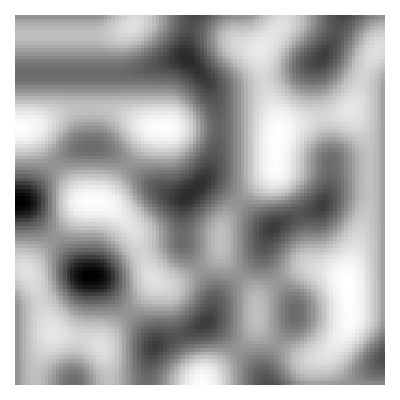
\includegraphics[width=.4\linewidth]{Images/perlin_noise}
	}
	\caption[Difference between noise patterns]{Difference between noise patterns.}
	\label{fig:noise_differences}
\end{figure}

\begin{figure}
	\centering
	\subfloat[Frequency 2]{%
	\label{fig:perlin_noise_2}%
	
\includegraphics[width=.3\linewidth]{Images/perlin_noise_2}
	}\quad
	\subfloat[Frequency 5]{%
	\label{fig:perlin_noise_5}%
	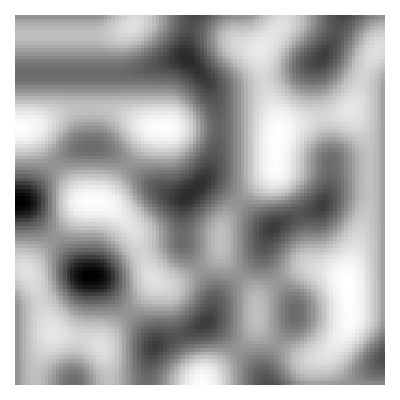
\includegraphics[width=.3\linewidth]{Images/perlin_noise}
	}\quad
	\subfloat[Frequency 20]{%
	\label{fig:perlin_noise_20}%
	
\includegraphics[width=.3\linewidth]{Images/perlin_noise_20}
	}
	\caption[Influence of frequency on Perlin noise]{Influence of frequency on Perlin noise patterns.}
	\label{fig:perlin_noise_frequencies}
\end{figure}

The second improvement is to use a regional mask. The original \gls{ba} applies a perturbation to the images as a whole. Every pixel will be perturbed with the same magnitude. This magnitude can be altered on a per-pixel basis when using a mask. Pixels that are further away from the target image will receive a larger perturbation than pixels that are already close to the corresponding pixel in the target. The mask $m$ is constructed according to equation \ref{eq:mask} based on the original image $x_{orig}$ and the adversarial image $x_{adv}$. It is then pixel-wise applied to the sampled perturbation in equation \ref{eq:mask_app}. The masked perturbation is normalized afterwards.\\ 

\begin{align}
m &= | x_{adv} - x_{orig}| \label{eq:mask}\\
\eta_{k} &= m \odot \eta_k; \eta_k = \frac{\eta_k}{\| \eta_k \|} \label{eq:mask_app}
\end{align}

This technique improves efficiency since the search space is significantly reduced. It is also possible to engineer masks for specific examples in order to incorporate other knowledge in the attack.\\

The final improvement is based on the idea of transfer attacks. A surrogate model is trained and will be used to calculate adversarial gradients. These gradients will then be used to bias the sampling direction for the orthogonal step. If the surrogate model does not closely resemble the defender, then the gradients will only hamper the speed of convergence of the attack instead of causing the attack to fail.

\begin{figure}
\centering
\tikzset{every picture/.style={line width=0.75pt}} %set default line width to 0.75pt        
\begin{tikzpicture}[x=0.75pt,y=0.75pt,yscale=-1,xscale=1]
%uncomment if require: \path (0,300); %set diagram left start at 0, and has height of 300

%Shape: Polygon Curved [id:ds5185908380685693] 
\draw  [fill={rgb, 255:red, 155; green, 155; blue, 155 }  ,fill opacity=0.5 ] (77.12,91.56) .. controls (95.12,69.56) and (136.12,35.56) .. (170.12,73.56) .. controls (204.12,111.56) and (165.12,154.56) .. (194.12,183.56) .. controls (223.12,212.56) and (189.12,259.56) .. (159.12,263.56) .. controls (129.12,267.56) and (33.12,279.56) .. (30.12,246.56) .. controls (27.12,213.56) and (79.12,216.56) .. (90.12,178.56) .. controls (101.12,140.56) and (59.12,113.56) .. (77.12,91.56) -- cycle ;
%Shape: Star [id:dp7170747564600322] 
\draw  [fill={rgb, 255:red, 0; green, 0; blue, 0 }  ,fill opacity=1 ] (122.62,191.06) -- (124.83,195.53) -- (129.76,196.24) -- (126.19,199.72) -- (127.03,204.63) -- (122.62,202.31) -- (118.22,204.63) -- (119.06,199.72) -- (115.49,196.24) -- (120.42,195.53) -- cycle ;
%Shape: Star [id:dp10477759386916752] 
\draw  [fill={rgb, 255:red, 0; green, 0; blue, 0 }  ,fill opacity=1 ] (94.62,14.06) -- (96.83,18.53) -- (101.76,19.24) -- (98.19,22.72) -- (99.03,27.63) -- (94.62,25.31) -- (90.22,27.63) -- (91.06,22.72) -- (87.49,19.24) -- (92.42,18.53) -- cycle ;
%Straight Lines [id:da2531323347021954] 
\draw    (94.62,21.56) -- (101.19,66.01) ;
\draw [shift={(101.62,68.98)}, rotate = 261.6] [fill={rgb, 255:red, 0; green, 0; blue, 0 }  ][line width=0.08]  [draw opacity=0] (8.93,-4.29) -- (0,0) -- (8.93,4.29) -- cycle    ;
%Straight Lines [id:da6594852147606747] 
\draw    (101.79,68.14) -- (91.03,74.6) ;
\draw [shift={(88.46,76.14)}, rotate = 329.04] [fill={rgb, 255:red, 0; green, 0; blue, 0 }  ][line width=0.08]  [draw opacity=0] (8.93,-4.29) -- (0,0) -- (8.93,4.29) -- cycle    ;
%Straight Lines [id:da6002841525279263] 
\draw    (88.46,76.14) -- (80.11,85.56) ;
\draw [shift={(78.12,87.81)}, rotate = 311.53] [fill={rgb, 255:red, 0; green, 0; blue, 0 }  ][line width=0.08]  [draw opacity=0] (8.93,-4.29) -- (0,0) -- (8.93,4.29) -- cycle    ;
%Straight Lines [id:da9148455444041863] 
\draw    (78.12,87.81) -- (71.8,97.16) ;
\draw [shift={(70.12,99.64)}, rotate = 304.06] [fill={rgb, 255:red, 0; green, 0; blue, 0 }  ][line width=0.08]  [draw opacity=0] (8.93,-4.29) -- (0,0) -- (8.93,4.29) -- cycle    ;
%Straight Lines [id:da47669503735159546] 
\draw    (70.12,99.64) -- (71.42,110.17) ;
\draw [shift={(71.79,113.14)}, rotate = 262.96] [fill={rgb, 255:red, 0; green, 0; blue, 0 }  ][line width=0.08]  [draw opacity=0] (8.93,-4.29) -- (0,0) -- (8.93,4.29) -- cycle    ;
%Straight Lines [id:da26104674623686774] 
\draw    (71.79,113.14) -- (76.37,123.08) ;
\draw [shift={(77.62,125.81)}, rotate = 245.27] [fill={rgb, 255:red, 0; green, 0; blue, 0 }  ][line width=0.08]  [draw opacity=0] (8.93,-4.29) -- (0,0) -- (8.93,4.29) -- cycle    ;
%Straight Lines [id:da9792015265988265] 
\draw    (77.62,125.81) -- (82.31,135.45) ;
\draw [shift={(83.62,138.14)}, rotate = 244.06] [fill={rgb, 255:red, 0; green, 0; blue, 0 }  ][line width=0.08]  [draw opacity=0] (8.93,-4.29) -- (0,0) -- (8.93,4.29) -- cycle    ;
%Straight Lines [id:da8018833944649997] 
\draw    (83.62,138.14) -- (87.84,148.69) ;
\draw [shift={(88.96,151.48)}, rotate = 248.2] [fill={rgb, 255:red, 0; green, 0; blue, 0 }  ][line width=0.08]  [draw opacity=0] (8.93,-4.29) -- (0,0) -- (8.93,4.29) -- cycle    ;
%Straight Lines [id:da7469050329272713] 
\draw    (88.96,151.48) -- (90.55,163.17) ;
\draw [shift={(90.96,166.14)}, rotate = 262.23] [fill={rgb, 255:red, 0; green, 0; blue, 0 }  ][line width=0.08]  [draw opacity=0] (8.93,-4.29) -- (0,0) -- (8.93,4.29) -- cycle    ;
%Straight Lines [id:da36931886382540347] 
\draw    (90.96,166.14) -- (88.57,177.7) ;
\draw [shift={(87.96,180.64)}, rotate = 281.69] [fill={rgb, 255:red, 0; green, 0; blue, 0 }  ][line width=0.08]  [draw opacity=0] (8.93,-4.29) -- (0,0) -- (8.93,4.29) -- cycle    ;
%Straight Lines [id:da3125285737899821] 
\draw    (87.96,180.64) -- (83.39,189.01) ;
\draw [shift={(81.96,191.64)}, rotate = 298.61] [fill={rgb, 255:red, 0; green, 0; blue, 0 }  ][line width=0.08]  [draw opacity=0] (8.93,-4.29) -- (0,0) -- (8.93,4.29) -- cycle    ;

%Curve Lines [id:da7332610230112269] 
\draw    (243,111.62) .. controls (297.92,70.43) and (367.93,279.11) .. (405,99.26) ;
%Shape: Star [id:dp6998768571531213] 
\draw  [fill={rgb, 255:red, 0; green, 0; blue, 0 }  ,fill opacity=1 ] (322.11,170.74) -- (325.14,176.87) -- (331.9,177.85) -- (327.01,182.62) -- (328.16,189.36) -- (322.11,186.18) -- (316.06,189.36) -- (317.22,182.62) -- (312.32,177.85) -- (319.09,176.87) -- cycle ;
%Straight Lines [id:da9467918607674688] 
\draw    (299.68,128.68) -- (331.29,83.87) ;
\draw [shift={(333.02,81.42)}, rotate = 125.2] [fill={rgb, 255:red, 0; green, 0; blue, 0 }  ][line width=0.08]  [draw opacity=0] (8.93,-4.29) -- (0,0) -- (8.93,4.29) -- cycle    ;
%Shape: Ellipse [id:dp07084957668985581] 
\draw  [color={rgb, 255:red, 128; green, 128; blue, 128 }  ,draw opacity=1 ][dash pattern={on 4.5pt off 4.5pt}] (264.94,181.03) .. controls (264.94,149.46) and (290.54,123.86) .. (322.11,123.86) .. controls (353.69,123.86) and (379.28,149.46) .. (379.28,181.03) .. controls (379.28,212.61) and (353.69,238.2) .. (322.11,238.2) .. controls (290.54,238.2) and (264.94,212.61) .. (264.94,181.03) -- cycle ;
%Straight Lines [id:da7547924674466151] 
\draw    (299.68,128.68) -- (326.52,124.97) ;
\draw [shift={(329.49,124.56)}, rotate = 172.13] [fill={rgb, 255:red, 0; green, 0; blue, 0 }  ][line width=0.08]  [draw opacity=0] (8.93,-4.29) -- (0,0) -- (8.93,4.29) -- cycle    ;
%Straight Lines [id:da7777022216727221] 
\draw    (329.49,124.56) -- (326.01,147.88) ;
\draw [shift={(325.57,150.85)}, rotate = 278.49] [fill={rgb, 255:red, 0; green, 0; blue, 0 }  ][line width=0.08]  [draw opacity=0] (8.93,-4.29) -- (0,0) -- (8.93,4.29) -- cycle    ;
%Straight Lines [id:da931484330606797] 
\draw [color={rgb, 255:red, 128; green, 128; blue, 128 }  ,draw opacity=1 ] [dash pattern={on 0.84pt off 2.51pt}]  (333.02,81.42) -- (329.49,124.56) ;


% Text Node
\draw (328.21,263) node   [align=left] {\begin{minipage}[lt]{96.27pt}\setlength\topsep{0pt}
classified correctly
\end{minipage}};
% Text Node
\draw (326.21,62) node   [align=left] {\begin{minipage}[lt]{96.27pt}\setlength\topsep{0pt}
classified incorrectly
\end{minipage}};
% Text Node
\draw (325.12,211.56) node   [align=left] {\begin{minipage}[lt]{68pt}\setlength\topsep{0pt}
original image
\end{minipage}};
% Text Node
\draw (112.21,256.14) node   [align=left] {\begin{minipage}[lt]{96.27pt}\setlength\topsep{0pt}
classified correctly
\end{minipage}};
% Text Node
\draw (106,13) node [anchor=north west][inner sep=0.75pt]   [align=left] {starting image};
% Text Node
\draw (56.21,116) node  [rotate=-286.01] [align=left] {\begin{minipage}[lt]{96.27pt}\setlength\topsep{0pt}
classified incorrectly
\end{minipage}};
% Text Node
\draw (120.12,225.56) node   [align=left] {\begin{minipage}[lt]{68pt}\setlength\topsep{0pt}
original image
\end{minipage}};
% Text Node
\draw (381.43,114.71) node   [align=left] {\begin{minipage}[lt]{68pt}\setlength\topsep{0pt}
1
\end{minipage}};
% Text Node
\draw (377.9,148.85) node   [align=left] {\begin{minipage}[lt]{68pt}\setlength\topsep{0pt}
2
\end{minipage}};
% Text Node
\draw (330,130) node [anchor=north west][inner sep=0.75pt]   [align=left] {$\displaystyle \epsilon $};
% Text Node
\draw (305,86) node [anchor=north west][inner sep=0.75pt]   [align=left] {$\displaystyle \eta $};


\end{tikzpicture}
\caption[Intuition of the Boundary Attack]{Intuition behind the Boundary Attack. On the left the path of the attack is shown. The first step is a projection onto the boundary, afterwards it follows the decision boundary of the class of the original image. Each arrow represents one iteration of the attack. On the right, the two different steps of each iteration can be seen. In the first step, a random direction is sampled and projected onto a sphere around the original image. The second step is to take a step towards the original image from this new position. Image inspired by \cite{boundary_attack}.}
\label{fig:boundary_attack_intuition}
\end{figure}

\section{HopSkipJumpAttack}
\gls{hsja} \cite{hsja}, like \gls{ba}, is a decision-based adversarial attack that starts from an adversarial input. The initial input is obtained in an identical manner as in \gls{ba}. \gls{hsja} is an iterative algorithm that consists of three steps.\\

The first step is a projection onto the decision boundary of the model under attack. This projection is carried out using a binary search. The second step is to estimate the direction of the gradient at the boundary. Different directions are sampled from a uniform distribution over a $d$-dimensional sphere, where $d$ is the input dimension. This random direction is added to the boundary point, generating a new query for the model. The results of these queries are combined to a gradient estimation~$\widetilde{\nabla S}$ using the Monte Carlo estimate of equation \ref{eq:monte_carlo_estimate}. In this equation $u_b$ are the random directions and $x_t$ is the boundary position. $B$ is the number of random directions that needs to be sampled. This number increases based on the current iteration of the attack to reduce the variance of the estimate. The function~$\phi_{x^*}$ returns 1 if the new position is adversarial and -1 if it is not adversarial. $\delta$ is a positive parameter determining the size of the $d$-dimensional sphere.

\begin{equation}\label{eq:monte_carlo_estimate}
\widetilde{\nabla S}(x_t,\delta) := \frac{1}{B} \sum_{b=1}^{B}\phi_{x^*}(x_t + \delta u_b)u_b
\end{equation}

Once the gradient has been estimated, the third and final operation is to take a step along this gradient. The step size is determined using a geometric progression scheme. These steps are iteratively repeated until the pre-set stopping criterion is met. Figure \ref{fig:hsja_intuition} represents the intuition behind \gls{hsja} in a graphical manner.\\

\gls{hsja} eclipses \gls{ba} and \gls{bba} both on median distance against queries and attack success rates using a limited amount of queries. The untargeted version of \gls{hsja} is able to compete with white box attacks on the ImageNet dataset \cite{imagenet}. It also performs similar or superior to white box attacks such as the C\&W attack \cite{cw_attack} when evaluated against defensive mechanisms such as defensive distillation \cite{defensive_distillation}, region-based classification \cite{region-based_classification} and adversarial training \cite{FGSM}.


\begin{figure}
\centering


\tikzset{every picture/.style={line width=0.75pt}} %set default line width to 0.75pt        

\begin{tikzpicture}[x=0.75pt,y=0.75pt,yscale=-1,xscale=1]
%uncomment if require: \path (0,300); %set diagram left start at 0, and has height of 300

%Curve Lines [id:da9704742483773781] 
\draw    (243,111.62) .. controls (297.92,70.43) and (367.93,279.11) .. (405,99.26) ;
%Shape: Star [id:dp26832364802919195] 
\draw  [fill={rgb, 255:red, 0; green, 0; blue, 0 }  ,fill opacity=1 ] (322.11,170.74) -- (325.14,176.87) -- (331.9,177.85) -- (327.01,182.62) -- (328.16,189.36) -- (322.11,186.18) -- (316.06,189.36) -- (317.22,182.62) -- (312.32,177.85) -- (319.09,176.87) -- cycle ;
%Shape: Ellipse [id:dp9511930412387599] 
\draw  [color={rgb, 255:red, 128; green, 128; blue, 128 }  ,draw opacity=1 ][dash pattern={on 4.5pt off 4.5pt}] (274.97,141.94) .. controls (274.97,120.26) and (292.54,102.69) .. (314.22,102.69) .. controls (335.9,102.69) and (353.48,120.26) .. (353.48,141.94) .. controls (353.48,163.63) and (335.9,181.2) .. (314.22,181.2) .. controls (292.54,181.2) and (274.97,163.63) .. (274.97,141.94) -- cycle ;
%Shape: Circle [id:dp5681517768642557] 
\draw  [fill={rgb, 255:red, 0; green, 0; blue, 0 }  ,fill opacity=1 ] (298,72.3) .. controls (298,71.03) and (299.03,70) .. (300.3,70) .. controls (301.57,70) and (302.6,71.03) .. (302.6,72.3) .. controls (302.6,73.57) and (301.57,74.6) .. (300.3,74.6) .. controls (299.03,74.6) and (298,73.57) .. (298,72.3) -- cycle ;
%Straight Lines [id:da06387380835189371] 
\draw    (300.3,72.3) -- (313.63,139) ;
\draw [shift={(314.22,141.94)}, rotate = 258.7] [fill={rgb, 255:red, 0; green, 0; blue, 0 }  ][line width=0.08]  [draw opacity=0] (8.93,-4.29) -- (0,0) -- (8.93,4.29) -- cycle    ;
%Straight Lines [id:da5011613685801404] 
\draw [color={rgb, 255:red, 155; green, 155; blue, 155 }  ,draw opacity=1 ][line width=0.75]  [dash pattern={on 0.84pt off 2.51pt}]  (314.22,141.94) -- (279.9,127.76) ;
\draw [shift={(278.05,127)}, rotate = 22.45] [fill={rgb, 255:red, 155; green, 155; blue, 155 }  ,fill opacity=1 ][line width=0.08]  [draw opacity=0] (12,-3) -- (0,0) -- (12,3) -- cycle    ;
%Shape: Boxed Line [id:dp5969211465757109] 
\draw [color={rgb, 255:red, 155; green, 155; blue, 155 }  ,draw opacity=1 ][line width=0.75]  [dash pattern={on 0.84pt off 2.51pt}]  (314.22,141.94) -- (327.54,107.28) ;
\draw [shift={(328.26,105.41)}, rotate = 111.02] [fill={rgb, 255:red, 155; green, 155; blue, 155 }  ,fill opacity=1 ][line width=0.08]  [draw opacity=0] (12,-3) -- (0,0) -- (12,3) -- cycle    ;
%Shape: Boxed Line [id:dp06580944891073615] 
\draw [color={rgb, 255:red, 155; green, 155; blue, 155 }  ,draw opacity=1 ][line width=0.75]  [dash pattern={on 0.84pt off 2.51pt}]  (314.22,141.94) -- (350.1,132.34) ;
\draw [shift={(352.03,131.82)}, rotate = 165.01] [fill={rgb, 255:red, 155; green, 155; blue, 155 }  ,fill opacity=1 ][line width=0.08]  [draw opacity=0] (12,-3) -- (0,0) -- (12,3) -- cycle    ;
%Shape: Boxed Line [id:dp5760742560965917] 
\draw [color={rgb, 255:red, 155; green, 155; blue, 155 }  ,draw opacity=1 ][line width=0.75]  [dash pattern={on 0.84pt off 2.51pt}]  (314.22,141.94) -- (340.03,168.65) ;
\draw [shift={(341.42,170.09)}, rotate = 225.98] [fill={rgb, 255:red, 155; green, 155; blue, 155 }  ,fill opacity=1 ][line width=0.08]  [draw opacity=0] (12,-3) -- (0,0) -- (12,3) -- cycle    ;
%Shape: Boxed Line [id:dp6962455418332032] 
\draw [color={rgb, 255:red, 155; green, 155; blue, 155 }  ,draw opacity=1 ][line width=0.75]  [dash pattern={on 0.84pt off 2.51pt}]  (314.22,141.94) -- (283.71,163.13) ;
\draw [shift={(282.07,164.27)}, rotate = 325.23] [fill={rgb, 255:red, 155; green, 155; blue, 155 }  ,fill opacity=1 ][line width=0.08]  [draw opacity=0] (12,-3) -- (0,0) -- (12,3) -- cycle    ;
%Straight Lines [id:da09211424476397356] 
\draw    (314.22,141.94) -- (345.36,106.42) ;
\draw [shift={(347.33,104.17)}, rotate = 131.23] [fill={rgb, 255:red, 0; green, 0; blue, 0 }  ][line width=0.08]  [draw opacity=0] (8.93,-4.29) -- (0,0) -- (8.93,4.29) -- cycle    ;
%Shape: Boxed Line [id:dp11391160549760482] 
\draw [color={rgb, 255:red, 155; green, 155; blue, 155 }  ,draw opacity=1 ][line width=0.75]  [dash pattern={on 0.84pt off 2.51pt}]  (314.22,141.94) -- (349.44,153.74) ;
\draw [shift={(351.34,154.37)}, rotate = 198.52] [fill={rgb, 255:red, 155; green, 155; blue, 155 }  ,fill opacity=1 ][line width=0.08]  [draw opacity=0] (12,-3) -- (0,0) -- (12,3) -- cycle    ;
%Shape: Boxed Line [id:dp7901030813069994] 
\draw [color={rgb, 255:red, 155; green, 155; blue, 155 }  ,draw opacity=1 ][line width=0.75]  [dash pattern={on 0.84pt off 2.51pt}]  (314.22,141.94) -- (302.05,106.86) ;
\draw [shift={(301.39,104.97)}, rotate = 70.87] [fill={rgb, 255:red, 155; green, 155; blue, 155 }  ,fill opacity=1 ][line width=0.08]  [draw opacity=0] (12,-3) -- (0,0) -- (12,3) -- cycle    ;
%Shape: Boxed Line [id:dp12912601709580973] 
\draw [color={rgb, 255:red, 155; green, 155; blue, 155 }  ,draw opacity=1 ][line width=0.75]  [dash pattern={on 0.84pt off 2.51pt}]  (314.22,141.94) -- (319.79,178.66) ;
\draw [shift={(320.09,180.64)}, rotate = 261.38] [fill={rgb, 255:red, 155; green, 155; blue, 155 }  ,fill opacity=1 ][line width=0.08]  [draw opacity=0] (12,-3) -- (0,0) -- (12,3) -- cycle    ;
%Shape: Boxed Line [id:dp15440737606551624] 
\draw [color={rgb, 255:red, 155; green, 155; blue, 155 }  ,draw opacity=1 ][line width=0.75]  [dash pattern={on 0.84pt off 2.51pt}]  (314.22,141.94) -- (301.49,176.83) ;
\draw [shift={(300.81,178.71)}, rotate = 290.05] [fill={rgb, 255:red, 155; green, 155; blue, 155 }  ,fill opacity=1 ][line width=0.08]  [draw opacity=0] (12,-3) -- (0,0) -- (12,3) -- cycle    ;
%Shape: Boxed Line [id:dp47011579703760575] 
\draw [color={rgb, 255:red, 155; green, 155; blue, 155 }  ,draw opacity=1 ][line width=0.75]  [dash pattern={on 0.84pt off 2.51pt}]  (314.22,141.94) -- (277.11,143.45) ;
\draw [shift={(275.11,143.53)}, rotate = 357.68] [fill={rgb, 255:red, 155; green, 155; blue, 155 }  ,fill opacity=1 ][line width=0.08]  [draw opacity=0] (12,-3) -- (0,0) -- (12,3) -- cycle    ;
%Shape: Boxed Line [id:dp3426945663084944] 
\draw [color={rgb, 255:red, 155; green, 155; blue, 155 }  ,draw opacity=1 ][line width=0.75]  [dash pattern={on 0.84pt off 2.51pt}]  (314.22,141.94) -- (345.13,121.35) ;
\draw [shift={(346.79,120.24)}, rotate = 146.33] [fill={rgb, 255:red, 155; green, 155; blue, 155 }  ,fill opacity=1 ][line width=0.08]  [draw opacity=0] (12,-3) -- (0,0) -- (12,3) -- cycle    ;

% Text Node
\draw (328.21,263) node   [align=left] {\begin{minipage}[lt]{96.27pt}\setlength\topsep{0pt}
classified correctly
\end{minipage}};
% Text Node
\draw (326.21,62) node   [align=left] {\begin{minipage}[lt]{96.27pt}\setlength\topsep{0pt}
classified incorrectly
\end{minipage}};
% Text Node
\draw (325.12,211.56) node   [align=left] {\begin{minipage}[lt]{68pt}\setlength\topsep{0pt}
original image
\end{minipage}};
% Text Node
\draw (304.6,75.3) node [anchor=north west][inner sep=0.75pt]   [align=left] {1};
% Text Node
\draw (262.33,131.33) node [anchor=north west][inner sep=0.75pt]   [align=left] {2};
% Text Node
\draw (346.33,92.67) node [anchor=north west][inner sep=0.75pt]   [align=left] {3};
\end{tikzpicture}
\caption[Intuition of the HopSkipJumpAttack]{Intuition behind the HopSkipJumpAttack. Each iteration consists of three steps. The first step is a projection onto the boundary. The second step is the estimation of the gradient at this point. This is done by sampling directions from a uniform distribution and querying the model under attack from this new position (grey arrows). The results are combined via the Monte Carlo estimate. The third and final step is to take a step along the estimated gradient. Image inspired by \cite{hsja}.}
\label{fig:hsja_intuition}
\end{figure}

\begin{figure}
\centering
\begin{tikzpicture}[xscale=0.75, yscale=0.75]
\definecolor{clr2}{RGB}{31,182,83}
\tikzset{
dot/.style = {circle, fill, minimum size=#1,
              inner sep=0pt, outer sep=0pt},
dot/.default = 6pt % size of the circle diameter 
}
\draw [fill={rgb, 255:red, 155; green, 155; blue, 155 }  ,fill opacity=0.5, draw=none] (0,7.5) -- (10,2.5) -- (10,10) -|cycle; % Fill above line

\path[name path=DB,draw, line width=0.5mm] (0,7.5) -- (10, 2.5); % Decision boundary

\begin{scope}[every node/.style={dot,thick,draw,anchor=base,fill=black}] % Circles
	\node[] (xo) at (3,3){}; %xo
	\node[] (xb) at (9,3){}; %xb
\end{scope}

\begin{scope}[red,line width=0.5mm]
\draw[] (xb) arc [
	start angle = 0,
	end angle = 180,
	radius = 3
];
\draw[] (xb) arc [
	start angle = 0,
	delta angle = -20,
	radius = 3
];
\draw[] (xo) arc [
	start angle = 180,
	delta angle = 20,
	radius = 3
];
\end{scope}

\begin{scope}[every node/.style={dot,thick,draw,anchor=base,fill=black}] % Circles
	\node[label=225:$x_o$] (xo) at (3,3){}; %xo
	\node[label=45:$x_b$] (xb) at (9,3){}; %xb
\end{scope}

\node[label=270:$u$] (xu) at (4.5,3){};
\node[label=180:$v$] (xv) at (3,4.5){};
\node[] (dl) at (3,1.5){};
\node[] (dr) at (9,1.5){};
\node[] (dal) at (3,0.5){};
\node[] (dar) at (7,0.5){};
\node[] (rpx) at (7,3){};
\path [-,line width=0.1mm, name path=guideline] (xo.east) edge (xb.west); % Guideline xo xb
\path [-latex, line width=0.5mm] (xo.east) edge (xu.west); % U arrow
\path [-latex, line width=0.5mm] (xo.north) edge (xv.south); % V arrow
\draw [spath/save=black, name path=blackarc, dashed] (rpx.center) arc (0:60:4);
\draw[dashed] (rpx) arc [start angle = 0, delta angle = -10, radius=4];
\path[spath/save=red, name path=redcircle] (xb) arc [
	start angle = 0,
	end angle = 180,
	radius = 3
];
\tikzset{
	spath/split at intersections={red}{black},
	spath/get components of ={black}\blackCpt,
}

\path[name intersections={of=DB and redcircle,by={Z, Z1}}];
\path [name intersections={of=blackarc and redcircle, by=intersect}];
\node[label=45:$z^*(\theta)$,dot,draw=red,anchor=base,fill=red] (i) at (intersect){};
\node[label=$z^*(\theta^*)$,dot,thick,draw=red,anchor=base,fill=red] (i2) at (Z1){};

\draw[spath/use={\getComponentOf\blackCpt{1}}, -latex, line width=0.5mm] node[right, pos=0.5] {$\theta$};
\path [dashed] (xo.center) edge (i.center);



\begin{scope}[color={rgb, 255:red, 31; green, 182; blue, 83}]
	\path [dashed] (dal.center) edge (xo.center);
	\path [dashed] (dr.center) edge (xb.center);
	\path [dashed] (dar.center) edge (rpx.center);
	\path [latex-latex, line width=0.5mm] (dl.center) edge node[fill=white] {$d$} (dr.center);
	\path [latex-latex, line width=0.5mm] (dal.center) edge node[fill=white] {$d(1-\alpha)$} (dar.center);
\end{scope}

\node[] (p) at (2,9){};
\draw [-latex, line width=0.5mm, blue, spath/save=normal] ($(xb)!(p)!(0,7.5)$) -- (p) node[]{$n$};
\draw [dashed, blue, line width=0.5mm] ($(xb)!(p)!(0,7.5)$) -- ($(xb)!(p)!(0,7.5) + (2,0)$);
\path[spath/save=dash] ($(xb)!(p)!(0,7.5) + (1.5,0)$) arc [start angle = 0, end angle = 90, radius = 1.5];
\tikzset{
	spath/split at intersections={normal}{dash},
	spath/get components of ={dash}\blueCpt,
}
\draw[spath/use={\getComponentOf\blueCpt{1}}, -latex, line width=0.5mm, blue] node[right, pos=0.5] {$\psi$};

\node[] at (8,9.5) {$\mathcal{O} \cap \mathcal{P}$};
\node[] (text) at (1,5.5) {$\partial\mathcal{O} \cap \mathcal{P}$};
\node[] (line) at (0.5,7.25) {};
\draw (text) to[out=0,in=-70] (line);
\end{tikzpicture}
\caption[Geographical configuration of SurFree]{•}
\label{fig:surfree}
\end{figure}


\section{Stateful defense}\label{sec:stateful_detection}
The defensive schemes discussed in section \ref{sec:adversarial_defenses} all operate on the query level. They try to detect and flag possible attacks based on a single query without taking other context into account. The stateful detection mechanism by Chen, Carlini and Wagner \cite{chen_stateful_2019} is different in this aspect. As the name suggests, it holds state of previously submitted queries. It is similar to the defenses that use proximity measurements, but the measurement is between queries instead of between the query and training data.\\

All queries submitted to the model equipped with a stateful detection mechanism are stored in a history buffer. Each user of the model has a distinct history buffer, where its queries are stored. These buffers can be bounded by time or number of queries depending on the resources available and the use case of the model. Each time a query is submitted to the model, the average distance to its $k$ nearest neighbors is calculated and if this distance is lower than a certain threshold, then the user gets flagged by the mechanism. Appropriate actions such as banning the account can be taken.\\

The distance metric is not calculated in input space. Each query is encoded by a deep similarity encoder \cite{deep_similarity_encoder} to an encoded space, typically of a lower dimension. In this encoded space, images which represent perceptually similar objects are clustered together. The advantage of the encoded space is twofold. Firstly, the dimension of the encoded space is smaller than the dimension of the input space. Therefore less space is needed to store the history buffers. Secondly, simpler distance metrics such as $L_2$-distance in input space can easily be evaded by an attacker. For example the $L_2$-distance can be significantly increased by simply rotating or shifting the input image.\\

The parameter $k$, the number of neighbors to consider is picked as follows. As the training data of the model consists of only benign queries, no attacks should be flagged when feeding the stateful detection mechanism with this data. To allow for some more leniency, a false positive rate of 0.1\% is still acceptable. For each value of $k$, a different threshold will be required to maintain the selected false positive rate. Larger values have the benefit of larger thresholds causing the defense to be more resilient, since attackers' images need to be more diverse. But $k$ is also the number of queries needed before an attack can be flagged. Therefore too large values for $k$ are disadvantageous. Smaller values also reduce computational cost. Chen, Carlini and Wagner set the value of $k$ to 50 for the CIFAR-10  dataset \cite{cifar}, since the thresholds increased sharply up to this value. Other datasets might require different values for $k$.

\section{PSO and distributed attacks}\label{sec:pso_and_distributed_attacks}
There have been several attempts to craft adversarial examples using an \gls{ea}. Previous attempts tried to reduce the number of queries needed to create a successful adversarial example by utilizing \glspl{ea} \cite{genattack,dong2019efficient,mosli2019they,audio_pso,distributed_pso_attack,suryanto2020}. \\

GenAttack \cite{genattack} and the similar efficient attack by Dong et al. \cite{dong2019efficient} use genetic algorithms in order to minimize the number of queries to the model. Both algorithms reduce the dimension of the search space to improve the efficiency of the attack. Once a promising perturbation is found in this lower dimensional space, it is upscaled using a bilinear transformation. By reducing the search space, the number of individuals in the genetic algorithm can be lowered, which in turn lowers the total amount of queries. GenAttack also uses annealing schemes to adaptively scale the parameters of the algorithm. This allows it to escape local optima and improve the adversarial example further. \\

AdversarialPSO \cite{mosli2019they} and the similar attack from \cite{audio_pso} use \gls{pso} as optimization routine on images and audio fragments respectively. Each particle represents a possible adversarial example. Both attacks use the standard rules of \gls{pso} as specified by \cite{pso} improved with a linearly decaying inertia weight \cite{inertia_weight}. The former attack also uses a constriction factor to avoid premature convergence \cite{constriction_factor}. While the latter solves this problem by generating new particles using a genetic algorithm when premature convergence is detected. Both algorithms rely on confidence scores to assign fitness values to certain positions in the search space. \gls{pso}-\gls{bba} \cite{distributed_pso_attack}, is similar to AdversarialPSO, but only relies on distances to determine fitness values. This attack can therefore also be used in decision-based settings instead of solely in score-based settings.\\

The idea behind the multi-group \gls{pso} attack \cite{suryanto2020} is to use multiple \gls{pso} swarms to escape local optima. The intuition behind it is inspired by the \gls{ddos} attack \cite{ddos}. The swarm is split into multiple smaller groups and each group is placed on a single node. The groups perform the standard \gls{pso} algorithm. The best position over all groups is communicated using a dedicated server. Each group submits its queries from its own node, tricking the defensive mechanism into thinking that multiple users are submitting queries. The authors state that this will ultimately result in less detections, but they have not evaluated this against a defensive scheme.\\


\bibliographystyle{unsrt}
\bibliography{bibliography}
\end{document}